\section{$\pi^{0}$ Mass Reconstruction in Data}
\label{sec:data_pi0}

% Samples
% We use two data samples in this study,
% \begin{itemize}
% \item 12 events, \texttt{PiZeroROI} + handscanning
% \item 6 events, NuMuCC filter + \texttt{PiZeroROI} + handscanning
% \end{itemize}
In this study, we investigate six events in data which pass
the NuMuCC filter, \texttt{PiZeroROI} selection and 
handscanning (ref.xx).\\
\\
All the shower-like PFParticles in the events in the data sample
are reconstructed as described in~\Cref{sec:reco}.
The subsequent step would be to find the two showers decaying from a 
$\pizero$ so that the $\pizero$ mass can be reconstructed according
to~\Cref{eq:pi0_mass}. \\
\\
% -----------------------------------------------------------------------
% Find the two showers: PFParticle hierarchy
Owing to the selection criteria of $\pizeroroi$, there is exactly one
neutrino-like PFParticle with two or three shower-like daughters in
each event.
Utilizing the hierarchy feature of Pandora outputs thereby becomes
the most straightforward strategy.
We loop over all the neutrino-like PFParticles (PDG code 12 or 14), 
identifying the one with at least two shower-like daughters.
In most of the events (five out of six), this kind of neutrino-like 
PFParticle has exactly two 
shower-like daughters, and the $\pizero$ mass is directly evaluated
from those two showers.
In the case that there are three shower-like daughters, we loop over
all the combinations of the showers and select the one with the largest
reconstructed $\pizero$ mass.
This approach gives us a reasonable result in our high-purity samples
as shown in~\Cref{fig:mpi0_data,table:mpi0_data}.
The values of nonzero $\pizero$ reconstructed mass are roughly
consistent with the peak value of the $\pizero$ distribution obtained
from single $\pizero$ MC events, \Cref{fig:mpi0_single_pi0}.\\
\\
% --------------------------------------------------------------------
% Figure: pi0 mass
\begin{figure}[htbp]
\begin{center}
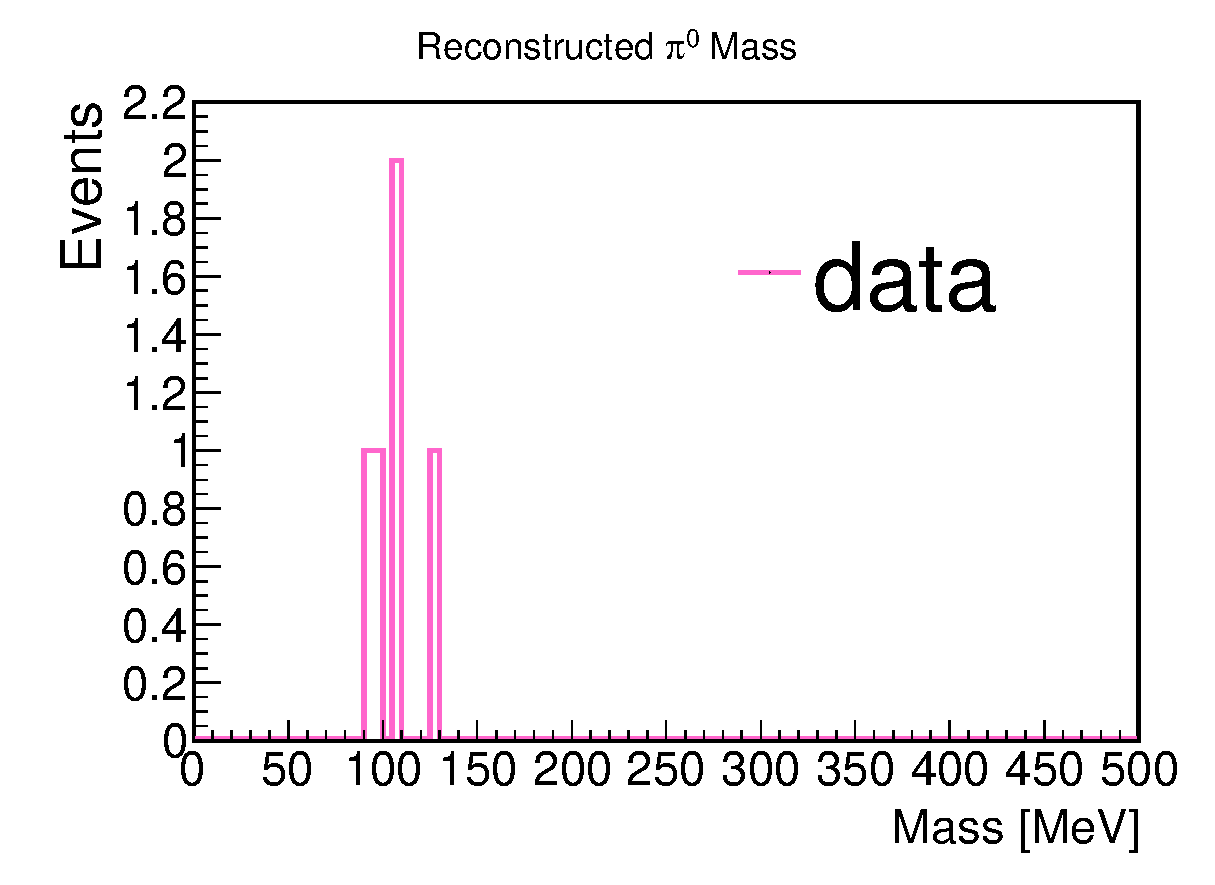
\includegraphics[width=0.75\textwidth]{figs/datapi0/data/RecoPi0Mass.eps}
\caption{Reconstructed $\pizero$ mass distribution from the six data events.
The event with zero reconstructed $\pizero$ mass is not included in this
figure.}
\label{fig:mpi0_data}
\end{center}
\end{figure}
% --------------------------------------------------------------------

%-------------------------------------------------------------------
\begin{table}[!h!tbp]
\begin{center}
\tabcolsep=10pt
\resizebox{0.95\textwidth}{!}{\begin{tabular}{ccccccc}
\hline
\hline
Run & Subrun & Event & Reco'ed E$_1$ (MeV) & Reco'ed E$_2$ (MeV) & $\cos(\theta_{12})$ & $m_{\pizero}$ (MeV) \\
\hline
6070 & 113 & 5680 & 104.09 & 31.32 & -0.77 & 104.09 \\
6145 &  16 & 814  & 57.69  & 54.92 & -0.49 & 97.27  \\
6058 &  94 & 4706 & 89.12  & 38.59 & -0.22 & 91.56  \\
5975 &  85 & 4262 & 109.36 & 89.61 & 0.15  & 129.11 \\
6015 &  69 & 3465 & 232.37 & 0.    & 0.98  & 0.     \\
6058 & 177 & 8877 & 60.02  & 51.33 & -0.91 & 108.52 \\
\hline
\hline
\end{tabular}}
\caption{The reconstructed quantities of the selected six events.}
\label{table:mpi0_data}
\end{center}
\end{table}
%-------------------------------------------------------------------


% -----------------------------------------------------------------------
% Ongoing issues
The most relevant topic on the current $\pizero$ mass reconstruction
in high-purity $\pizero$ samples is the deficiency in the reconstructed
energy, which shifts the peak of the $\pizero$ mass distribution, as
demonstrated in~\Cref{fig:mpi0_single_pi0}.
The same feature is obviously seen in the studies with the single electron
and photon MC samples in~\Cref{sec:single_em}.
We discuss the ongoing studies and possible corrections in~\Cref{sec:ongoing}.


